\documentclass{article}\usepackage[]{graphicx}\usepackage[]{xcolor}
% maxwidth is the original width if it is less than linewidth
% otherwise use linewidth (to make sure the graphics do not exceed the margin)
\makeatletter
\def\maxwidth{ %
  \ifdim\Gin@nat@width>\linewidth
    \linewidth
  \else
    \Gin@nat@width
  \fi
}
\makeatother

\definecolor{fgcolor}{rgb}{0.345, 0.345, 0.345}
\newcommand{\hlnum}[1]{\textcolor[rgb]{0.686,0.059,0.569}{#1}}%
\newcommand{\hlstr}[1]{\textcolor[rgb]{0.192,0.494,0.8}{#1}}%
\newcommand{\hlcom}[1]{\textcolor[rgb]{0.678,0.584,0.686}{\textit{#1}}}%
\newcommand{\hlopt}[1]{\textcolor[rgb]{0,0,0}{#1}}%
\newcommand{\hlstd}[1]{\textcolor[rgb]{0.345,0.345,0.345}{#1}}%
\newcommand{\hlkwa}[1]{\textcolor[rgb]{0.161,0.373,0.58}{\textbf{#1}}}%
\newcommand{\hlkwb}[1]{\textcolor[rgb]{0.69,0.353,0.396}{#1}}%
\newcommand{\hlkwc}[1]{\textcolor[rgb]{0.333,0.667,0.333}{#1}}%
\newcommand{\hlkwd}[1]{\textcolor[rgb]{0.737,0.353,0.396}{\textbf{#1}}}%
\let\hlipl\hlkwb

\usepackage{framed}
\makeatletter
\newenvironment{kframe}{%
 \def\at@end@of@kframe{}%
 \ifinner\ifhmode%
  \def\at@end@of@kframe{\end{minipage}}%
  \begin{minipage}{\columnwidth}%
 \fi\fi%
 \def\FrameCommand##1{\hskip\@totalleftmargin \hskip-\fboxsep
 \colorbox{shadecolor}{##1}\hskip-\fboxsep
     % There is no \\@totalrightmargin, so:
     \hskip-\linewidth \hskip-\@totalleftmargin \hskip\columnwidth}%
 \MakeFramed {\advance\hsize-\width
   \@totalleftmargin\z@ \linewidth\hsize
   \@setminipage}}%
 {\par\unskip\endMakeFramed%
 \at@end@of@kframe}
\makeatother

\definecolor{shadecolor}{rgb}{.97, .97, .97}
\definecolor{messagecolor}{rgb}{0, 0, 0}
\definecolor{warningcolor}{rgb}{1, 0, 1}
\definecolor{errorcolor}{rgb}{1, 0, 0}
\newenvironment{knitrout}{}{} % an empty environment to be redefined in TeX

\usepackage{alltt}
\title{\textbf{R Lab One}}
\author{\textbf{Katherine Wolf}\\ Introduction to Causal Inference (PH252D)\\ \today}
\date{}

% list of latex packages you'll need
\usepackage{float}  % for tables
\usepackage{mathtools}  % for mathematical symbols
\usepackage{bm}  % to bold mathematical symbols like betas
\usepackage{scrextend}  % to indent subsections
\usepackage{xltxtra}
\usepackage{fontspec}
\usepackage{xunicode}
\usepackage[skip=0.5\baselineskip]{caption}  % control caption printing space
\usepackage{longtable}
\usepackage{amsmath}
\usepackage{amsfonts}
\usepackage{bm}
\usepackage{caption}
\usepackage[shortlabels]{enumitem}
\usepackage{txfonts}
\usepackage{dejavu}

% set fonts
\setmainfont{Georgia}
\setsansfont[Scale=MatchLowercase]{Arial}  % sets the sans font
\setmonofont[Scale=MatchLowercase]{DejaVuSansMono}  % sets the monospace font

% make special code formatting
\NewDocumentCommand{\codeword}{v}{%
  \texttt{{#1}}%
}

% set the margins of the document
\usepackage[top=1in, bottom=1in, left=.5in, right=.5in]{geometry}
\setlength\parindent{0pt}



% end the preamble and begin the document
\IfFileExists{upquote.sty}{\usepackage{upquote}}{}
\begin{document}

\maketitle

\section{Background Story}

\section{Steps 1-5 of the Roadmap}

  \subsection{Step 1: Causal model representing real knowledge}
  
  \begin{enumerate}[label=\textbf{\alph*.}]

    \item \textbf{Draw the accompanying directed acyclic graph (DAG).}
    
\begin{knitrout}
\definecolor{shadecolor}{rgb}{0.969, 0.969, 0.969}\color{fgcolor}
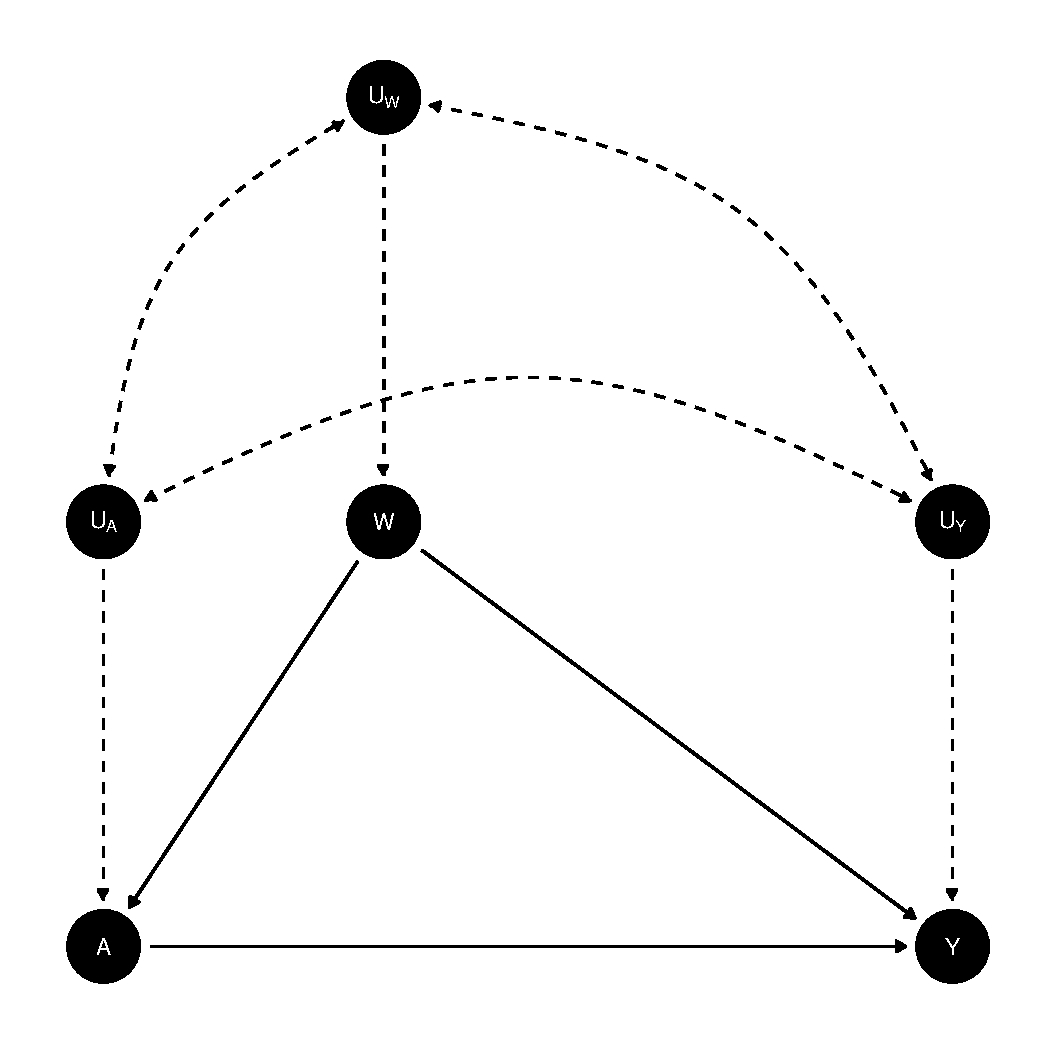
\includegraphics[width=4in]{figure/unnamed-chunk-2-1} 

\end{knitrout}
    

    \item \textbf{Are there any exclusion restrictions? Recall we are working with recursive (time-ordered) structural causal models.}
    
    \item \textbf{Are there any independence assumptions on the distribution of unmeasured factors $\mathbb{P}_U$?}

  \end{enumerate}
  
  \subsection{Step 2: Counterfactuals and causal parameter}
  
  \begin{enumerate}[label=\textbf{\alph*.}]
  
    \item \textbf{Define the counterfactual outcomes of interest with formal notation and in words.}
    
    \item \textbf{How are counterfactuals derived?}
    
    \item \textbf{Suppose we are interested in the average treatment effect. Specify the target causal parameter. Use formal notation as well as explain in words.}
 
  \end{enumerate}
  
  \subsection{Step 3: Observed data and link to causal}
  
  \begin{enumerate}[label=\textbf{\alph*.}]
  
    \item \textbf{Specify the link between the SCM and the observed data.}
    
    \item \textbf{What restrictions, if any, does the SCM place on the allowed distributions for the observed data? (Recall d-separation.)}
    
    \item \textbf{What notation do we use to denote the true (but unknown) distribution of the observed data and the statistical model?}
  
  \end{enumerate}
  
  \subsection{Steps 4-5: Identification and statistical estimand}
  
  \begin{enumerate}[label=\textbf{\alph*.}]
  
    \item \textbf{Using the backdoor criterion, assess identifiability.}
    
    \item \textbf{If the target causal parameter is not identified, under what assumptions would it be?}
    
    \item \textbf{What notation is used to denote the original SCM augmented with additional assumptions needed for identifiability?}
    
    \item \textbf{Specify the target parameter of the observed data distribution (the statistical estimand).}
    
    \item \textbf{What is the relevant positivity assumption? Is it reasonable here?}
  
  \end{enumerate}
  
\pagebreak

\section{Bonus: Identifying the Mean Outcome Under a Dynamic Intervention}

\begin{enumerate}[label=\textbf{\arabic*.}]
  
  \item \textbf{Explain why (1) holds using properties of conditional expectations. Given access to the full population and the ability to implement intervention \textit{d}, what does (1) tell you about how you could compute $\mathbb{E}_{U,X}[Y_d]$?}
  
  \item \textbf{Explain why (2) holds using properties of conditional expectations and the fact that $Y_d \Perp A|W_1, W_2$ under our convenience assumptions for the backdoor criterion made in Question 4 of Section 2.}
  
  \item \textbf{Explain why (3) holds. What does this mean in terms of the RUTF example?}
  
  \item \textbf{Explain why (4) holds. What does this mean in terms of the RUTF example?}
  
\end{enumerate}

\pagebreak

\section{A Specific Data-Generating Process}

  \subsection{Closed form evaluation on the target parameter}
  
    \begin{enumerate}[label=\textbf{\arabic*.}]
    
      \item \textbf{Evaluate the target causal parameter $\psi^F(\mathbb{P}_{U,X})$ in closed form (i.e., by hand) for this data generating process.}
      
      \item \textbf{Interpret $\psi^F(\mathbb{P}_{U,X})$.}
  
    \end{enumerate}
    
  \subsection{Translating this data generating process for $\mathbb{P}_{U,X}$ into simulations, generating counterfactual outcomes and evaluating the target causal parameter.}
  
    \begin{enumerate}[label=\textbf{\arabic*.}]
    
      \item \textbf{First set the seed to 252.}
      
      \item \textbf{Set $n = 50,000$ as the number of independent and identically distributed draws from the data-generating process.}
      
      \item \textbf{Simulate the background factors $U$.}
      
      \item \textbf{Evaluate the structural equations $F$ to deterministically generate the endogenous nodes $X$.}
      
      \item \textbf{Intervene to set the supplement to RUTF $(A = 1)$ and generate counterfactual outcomes $Y_1$ for $n$ units. Then intervene to set the supplement to the standard $(A = 0)$ and generate counterfactual outcomes $Y_0$ for $n$ units.}
      
      \item \textbf{Create a data frame $X$ to hold the values of the endogenous factors $(W_1, W_2, A, Y)$ and the counterfactual outcomes $Y_1$ and $Y_0$. The rows are the n children and the columns are their characteristics. Use the head and summary to examine the resulting data.}
      
      \item \textbf{Evaluate the causal parameter $\psi^F(\mathbb{P}_{U,X})$ for this population of 50,000 units.}
  
    \end{enumerate}

\pagebreak
  
\section{Defining the Target Causal Parameter with a Working Marginal Structural Model}

\begin{enumerate}[label=\textbf{\arabic*.}]

  \item \textbf{For $n = 5,000$ children, generate the exogenous factors $U$ and the pre-intervention covariates $(V, W1, W2)$. Then set $A = 1$ to generate the counterfactual weight gain under RUTF $Y_1$. Likewise, set $A = 0$ to generate the counterfactual weight gain under the standard supplement $Y_0$.}
  
  \item \textbf{Create a data frame} \codeword{X.msm} \textbf{consisting of age $V$, the set treatment levels $a$, and the corresponding outcomes $Y_a$.}
  
  \item \textbf{Evaluate the target causal parameter.}
  
  \item \textbf{Interpret the results.}

\end{enumerate}
      
\end{document}
